\chapter{Architecture}

\begin{figure}
	\centering
	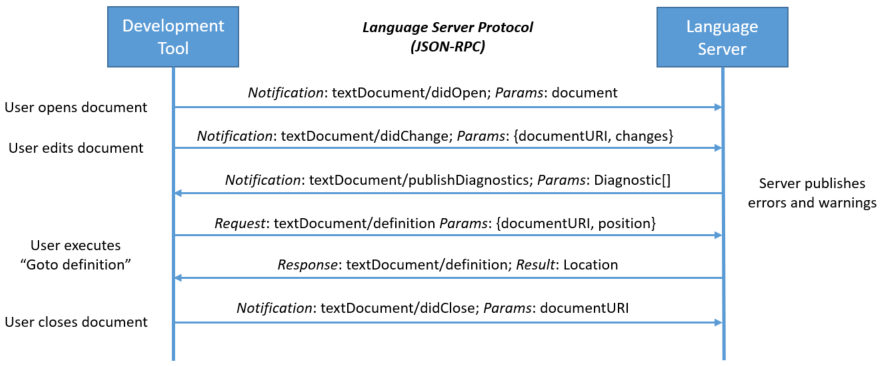
\includegraphics[width=\textwidth]{img/language-server-sequence}
	\caption{LSP session example}
	\label{fig04:LSP}
\end{figure}

\begin{figure}
	\centering
	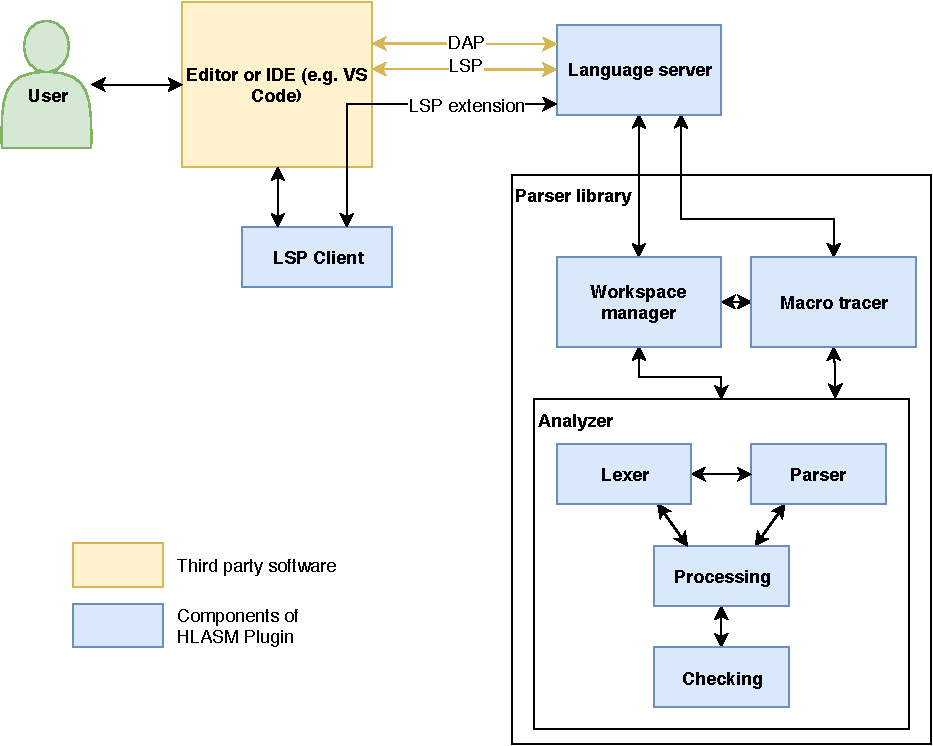
\includegraphics[width=\textwidth]{img/hlasm_architecture}
	\caption{The architecture of HLASM Plugin}
	\label{fig04:arch}
\end{figure}



The architecture is based on the way modern code editors and IDEs are extended to support additional languages. We chose to implement Language Server Protocol \footnote{https://microsoft.github.io/language-server-protocol/} (LSP), which is supported by majority of contemporary editors.

In LSP the two parties who communicate are called \emph{client} and \emph{language server}. A simple example is displayed in Figure~\cref{fig04:LSP} The client runs as a part of an editor. Language server may be standalone application, that is connected to the client by a pipe or TCP. All language-specific user actions are transformed into standard LSP messages and sent to the language server, which analyses the source code and sends back response, which is then interpreted and presented to the user in editor-specific way. This architecture makes possible to have only one LSP client implementation for each code editor which may be reused by all programming languages. And vice versa, every language server may be easily used by any editor that has an implementation of LSP client.

To add support for HLASM we have to implement LSP language server and write thin extension to an editor, which will use already existing implementation of LSP client. To implement source code highlighting, we have to extend the protocol with a new notification to transfer information from language server to VS Code client, which is extended to highlight code in editor based on the incoming custom notifications.

This chapter presents decomposition of the project into smaller components and describes their relations. The main two components are language server --- an executable application that uses parser library. The overall architecture is pictured in Figure~\cref{fig04:arch}.

\section{Language server}

The responsibility of the Language server component is to maintain the LSP session, convert the JSON messages and use the parser library to execute them. The functionality includes:
\begin{itemize}
    \item To read LSP messages from standard input or TCP and write responses.
    \item To parse JSON RPC to C++ structures so they can be further used.
    \item To serialize C++ structures into JSON, so it can be sent back to client.
    \item Implement asynchronous request handling: e.g. when user makes several consecutive changes to a source code, it is not needed to parse every change, only the final version.
\end{itemize}

\section{Parser library}

Parser library is the core of the project --- it encapsulates all parsing capabilities, keeps track of opened files in the editor and provides information about them. It has API based on LSP --- every relevant request and notification has corresponding method in parsing library. The API includes:

\begin{itemize}
	\item Implementation of text synchronization notifications (didOpen, didChange, didClose), which inform the library about files that are currently opened in the editor and their exact contents.
	\item Implementation of workspace management notifications (DidChangeWorkspaceFolders): many editors have possibilities to open more workspaces in the same time, the parser library supports this too. Workspace is basically just a folder which contains related source codes. Workspaces help parser library find macro and copy files.
	\item A method to consume DidChangeWatchedFiles notification which makes it possible to react to workspace changes that were not made by the user in editor, but still may affect the parsing. For example when user deletes an external macro file, the parser library should react by reporting that it cannot find the macro.
	\item Implementation of diagnostics publishing (publishDiagnostics notification). A diagnostic is used to indicate a problem with source files, such as compiler error or warning. The parser library provides a callback to let language server know that diagnostics have changed.
	\item Callback for highlighting information provision.
	\item Implementation of language feature requests (definition, references, hover, completion), which provide information needed for proper reaction of the editor on user actions.
	
\end{itemize}

The parser library is further decomposed into smaller components.

\subsection{Analyser}

Analyser is able to process a single HLASM file. The processing includes:
\begin{itemize}
 \item Recognition of statements and their parts (lexing and parsing).
 \item Interpretation of instructions that should be executed in compile time.
 \item Check whether the HLASM source code is well-formed.
 \item Report problems with the source by producing LSP diagnostics.
 \item Provide highlighting and LSP information.
\end{itemize}

A HLASM file may have dependencies --- other files, that define macros or files brought in by COPY instruction. The dependencies are only discovered during processing of files, so it is not possible to provide the files beforehand. The analyser must get a callback that would find a file with specified name, parse its contents and return it as list of parsed statements. 

To sum up, analyser has pretty simple API: it takes the contents of a source file by common string and a callback that can parse external files with specified name. It provides list of diagnostics connected with the file, highlighting and list of symbol definitions, etc.

The analyser is further decomposed into 4 components.

\subsubsection{Lexer}

Lexer task is to read source string and break it into tokens --- small pieces of text with special meaning. The most important features of the lexer:
\begin{itemize}
	\item Check whether all characters ale valid in HLASM source
	\item Each token has location in the source text
	\item Ability to jump in the source file backward and forward is necessary for implementation of instructions like AGO and AIF.
\end{itemize}

\subsubsection{Parser}

Parser component takes the stream of tokens the lexer produces and recognises HLASM statements according to syntax. To accomplish this, a parser generator tool Antlr 4 \footnote{https://www.antlr.org} is used.

Antlr takes as input grammar (written in antlr-specific language) that specifies syntax of HLASM language and generates source code (in C++) for recognizer, which is able to tell whether input source code is valid or not. Moreover, it is possible to assign a piece of code that executes every time a grammar rule is matched by the recognizer to further process the matched piece of code.



\subsubsection{Processing}

Results of the parser component are further analysed in processing component. The most important features are:

\begin{itemize}
	\item CA instructions are interpreted here: that results in modifying lexer state (moving back and forth in the input file).
	\item Substitution of variable symbols. After the substitution, the statement must be reparsed in the lexer and parser again.
	\item Interpretation of assembler instructions to evaluate ordinary symbols.
	\item MACRO and COPY expansion.
\end{itemize}

\subsubsection{Checking}
After a statement is fully processed, all operands of each instruction are known, it needs to be checked. There are over 2000 machine instructions with variable number of operands and various restrictions on those operands --- some of them take only positive numbers, only numbers that are in specific range or take address only. Checking component takes an instruction and list of its operands and returns list of problems in form of LSP diagnostics.


\subsection{Workspace manager}

Workspace manager responsibility is to keep workspaces and files representation in parser library exactly the same as the user sees in the editor. Further, it starts analyser when needed, manages workspace configuration and provides external macro and copy libraries to analyser.

\section{VS code extension}

The VS Code extension component ensures seamless integration with the editor. Its functions are:

\begin{itemize}
	\item To start LSP client that comes with VS Code, HLASM language server and create connection between them.
	\item To implement server-side highlighting, which extends the LSP protocol.
	\item To improve user experience regarding continuations and fixed length line source codes.
\end{itemize}


\section{Macro tracer}
Macro tracer enables the user to trace the compilation of HLASM source code in a way similar to common debugging. That is the reason why we chose to implement Debug Adapter Protocol \footnote{https://microsoft.github.io/debug-adapter-protocol/} (DAP). It is very similar to LSP, so most of the code implementing LSP in the language server component may be reused for both protocols.

The language server component communicates with macro tracer component in parser library. Its API mirrors the requests and events of DAP. The most important features to implement are:

\begin{itemize}
	\item Launch, continue, next, stepIn and disconnect requests allow user to control the flow of the compilation.
	\item SetBreakpoints get information about breakpoints that the user has placed in the code.
	\item Threads, StackTrace, Scopes and Variables requests to allow the DAP client to retrieve information about current processing stack (stack of nested macros and copy instructions), available variable symbols and their values.
	\item Stopped, exited and terminated events to let the DAP client know about state of traced source code.
\end{itemize}

Macro traces communicates with the workspace manager to retrieve contents of traced files. Further, it starts analysing the source file in a separate thread and get callbacks from the analyser before a statement is processed. In the callback, tracer puts the thread to sleep and wait for user interaction. During this time, it is possible to retrieve all variable and stack information from the processing to show it to the user.
